\chapter{Results \& Discussion}
\section{Single model parameters}
\subsection{Choosing between regressors and classifiers}

Initially, Morgan fingerprints with a radius of 2 and a size of 2048 bits were taken as fingerprints for predicting docking hits.
The first goal was to determine whether classifiers or regressors have better predicting ability.
Fig. \ref{Regressors} and Fig. \ref{Classifiers} show that most regressors perform better than classifiers.\\

Baseline models, such as RandomUniformRegressor and RandomGaussianRegressor should not be included in consideration, because they are baseline models which are necessary for setting the lower bound of recall score.
The analysis of recall score of different types of machine learning models have shown that is is preferable to pick a model for iterative algorithm from regressors.\\

\begin{figure}[h]
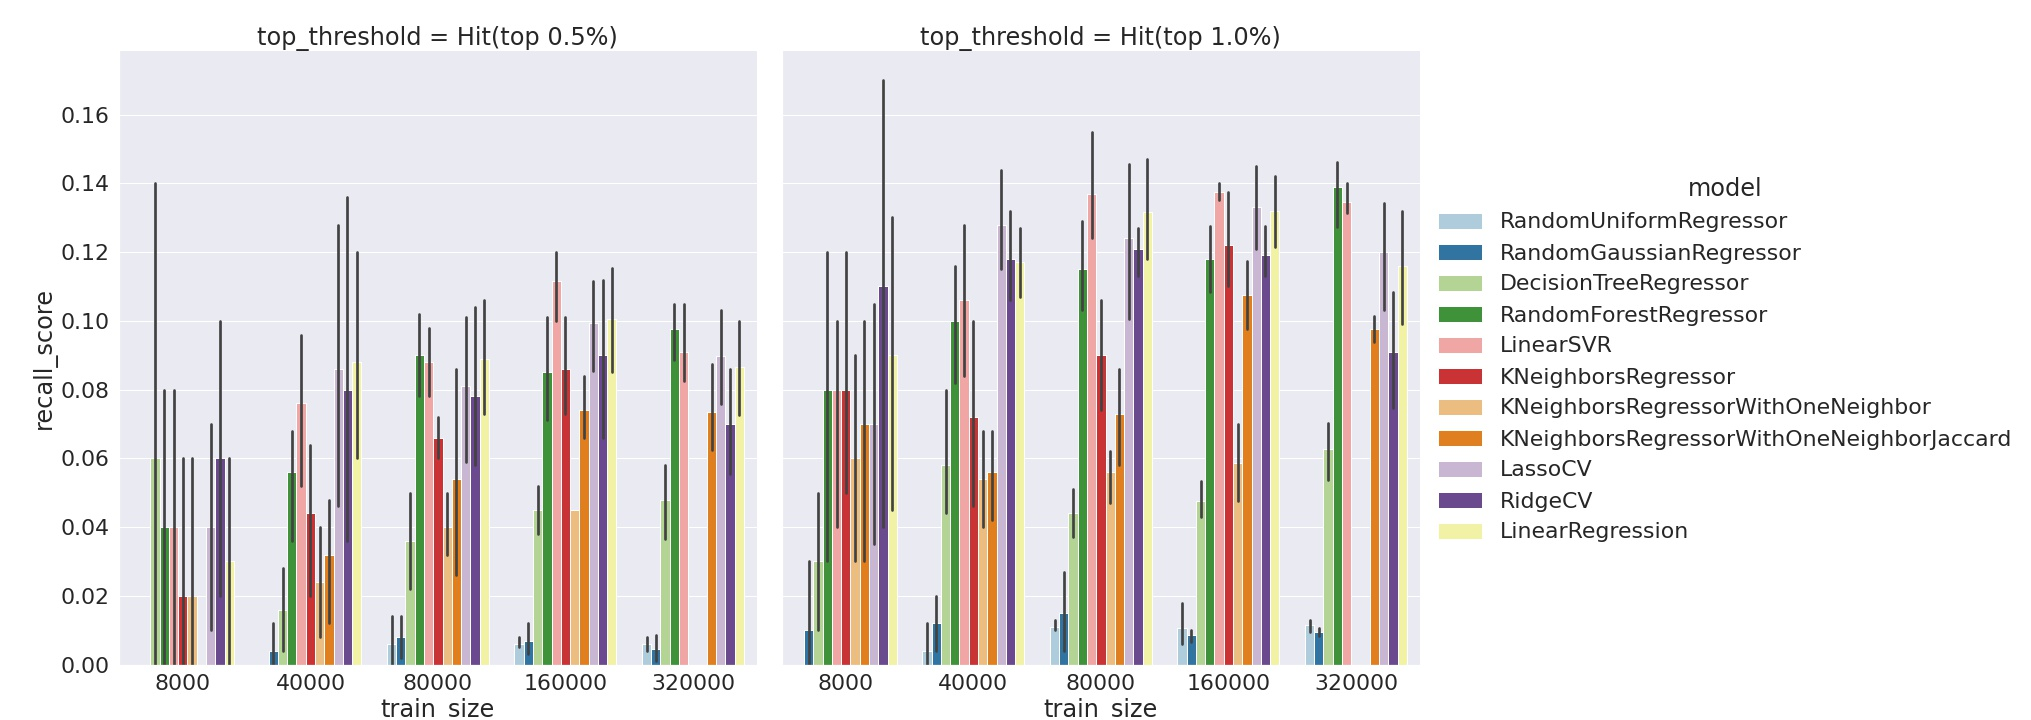
\includegraphics[scale=0.25]{Images/MorganRadius2Size2048Regressor1.jpg} 
\caption{Recall score of regressors trained on Morgan fingerprints with radius 2 and size 2048 (models are trained on the docking scores obtained for target 4eiy)}
\label{Regressors}
\newpage
\end{figure}

\begin{figure}[h]
\centering
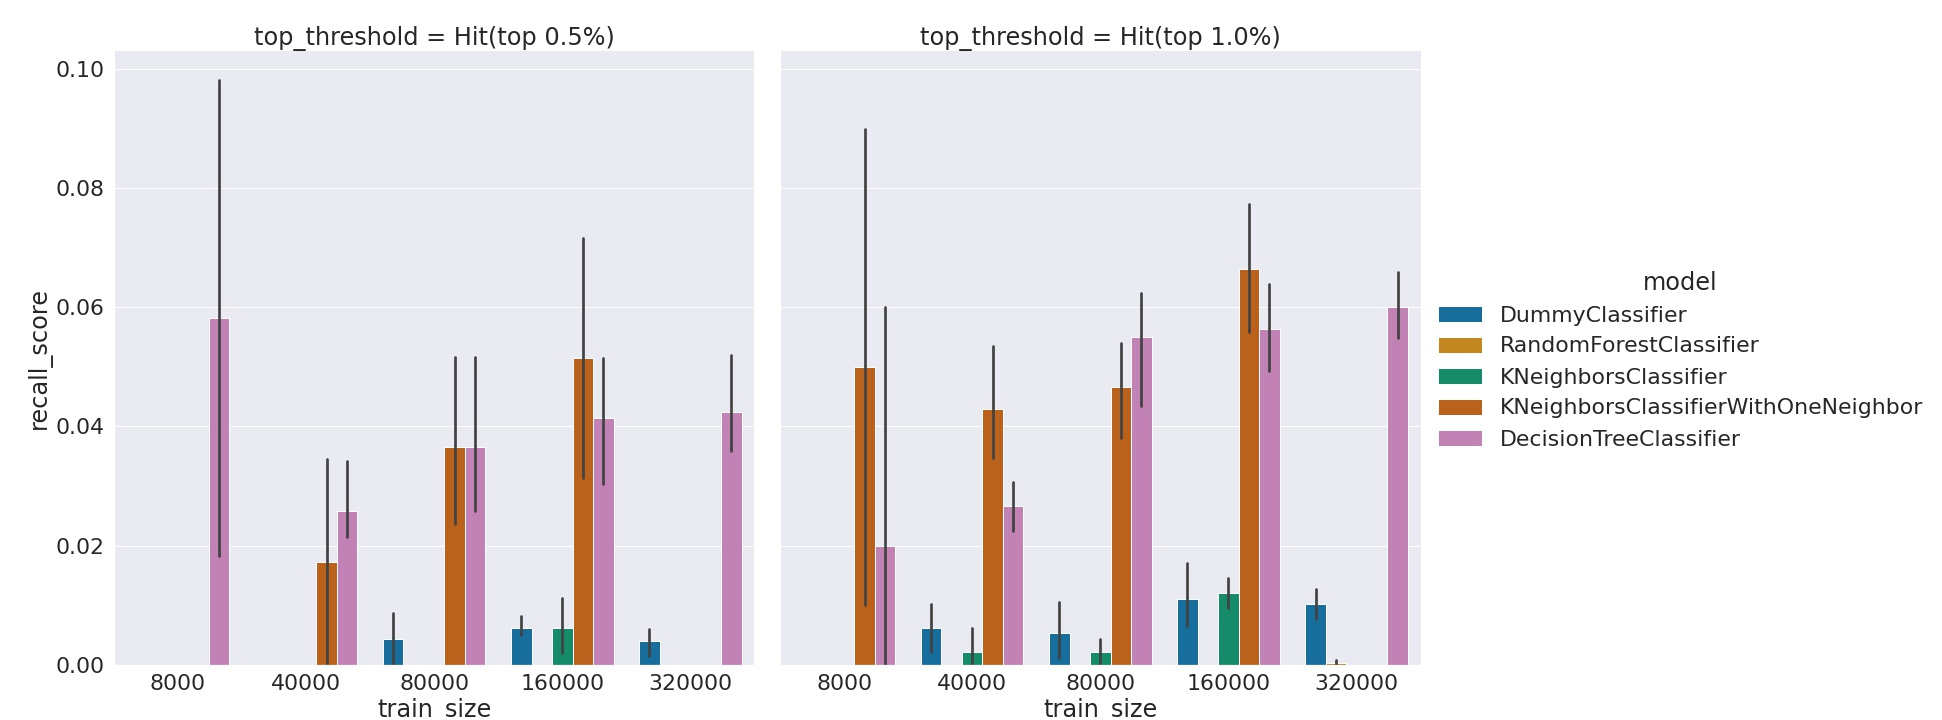
\includegraphics[scale=0.25]{Images/MorganRadius2Size2048Classifier1.jpg} 
\caption{Recall score of classifiers trained on Morgan fingerprints with radius 2 and size 2048 (models are trained on the docking scores obtained for target 4eiy)}
\label{Classifiers}
\end{figure}

Among all regressors, linear methods are favorable: they have high recall score while requiring only a couple of minutes to train and make prediction.
Due to these properties, linear models are suitable for iterative algorithm. However, not all linear models perform the same way on targets 4eiy and 5zty. The information about models trained on 8,000 compounds is presented in Table. \ref{recalls}.\\

As one may notice, linear regression is fine for making predictions for target 4eiy; however it performs poorly on 5zty. 
Hereby, linear regression may be chosen for predicting docking scores for 4eiy target, but not for 5zty.
Considering second target, RidgeCV performs better than linear regression, still needing a few minutes to work.
Both models are to be employed in the iterative algorithm and to be compared.
Moreover, linear support vector regressions is to be studied further as the fastest algorithm which still obtains high recall score.\\

% Please add the following required packages to your document preamble:
% \usepackage{multirow}
% \usepackage[table,xcdraw]{xcolor}
% If you use beamer only pass "xcolor=table" option, i.e. \documentclass[xcolor=table]{beamer}
\begin{table}[H]
\centering
\begin{tabular}{@{}|l|r|r|r|r|r|@{}}
\hline
\multicolumn{1}{|c|}{}                                 & \multicolumn{1}{c|}{}                                & \multicolumn{2}{c|}{\textbf{recall\_score}}     & \multicolumn{2}{c|}{\textbf{time}}              \\ \cline{3-6} 
\multicolumn{1}{|c|}{\multirow{-2}{*}{\textbf{model}}} & \multicolumn{1}{c|}{\multirow{-2}{*}{\textbf{type}}} & \multicolumn{1}{c|}{\textbf{4eiy}} & \multicolumn{1}{c|}{\textbf{5zty}} & \multicolumn{1}{c|}{\textbf{4eiy}} & \multicolumn{1}{c|}{\textbf{5zty}} \\ \hline
RidgeCV & regressor & 0.14700 & 0.11150 &   00:04:23 &   00:00:19       \\ \hline
\begin{tabular}[c]{@{}l@{}}LinearRegression\\ (weight=100)\end{tabular}                                              & regressor                                                                    & 0.14375                           & 0.03575                           &   00:02:37         &   00:00:17          \\ \hline
\begin{tabular}[c]{@{}l@{}}LinearRegression\\ (weight=50)\end{tabular}                                                & regressor                                                                    & 0.14375                           & 0.03575                           &   00:02:43          &   00:00:17          \\ \hline
\begin{tabular}[c]{@{}l@{}}LinearRegression\\ (weight=20)\end{tabular}                                               & regressor                                                                    & 0.13900                           & 0.03575                           &   00:02:33        &   00:00:17          \\ \hline
\begin{tabular}[c]{@{}l@{}}LinearRegression\\ (weight=10)\end{tabular}                                                & regressor                                                                    & 0.13475                           & 0.03575                           &   00:02:19          &   00:00:16        \\ \hline
Ridge                                                                          & regressor                                                                    & 0.13400                           & 0.10000                           &   00:03:57          &   00:00:15        \\ \hline
LinearSVR                                                                      & regressor                                                                    & 0.13350                           & 0.10125                           &   00:00:41          &   00:00:13            \\ \hline
LinearRegression                                                               & regressor                                                                    & 0.13263                           & 0.09925                           &   00:03:54       &   00:00:16        \\ \hline
LassoCV                                                                        & regressor                                                                    & 0.13250                           & 0.13150                           &   00:09:25       &   00:01:16        \\ \hline
RandomForestRegressor                                                          & regressor                                                                    & 0.12475                           & 0.10600                           &   00:07:23         &   00:03:45         \\ \hline
KNeighborsRegressor                                                            & regressor                                                                    & 0.09450                           & 0.07125                           &   00:05:18        &   00:01:08        \\ \hline
\begin{tabular}[c]{@{}l@{}}KNeighborsRegressor\\ (1 neighbour, metric=jaccard)\end{tabular}                                  & regressor                                                                    & 0.07775                           & 0.05875                           &   00:02:15         &   00:01:29         \\ \hline
DecisionTreeRegressor                                                          & regressor                                                                    & 0.07575                           & 0.05075                           &   00:03:41          &   00:00:17         \\ \hline
DecisionTreeClassifier                                                         & classifier                                                                   & 0.06715                           & 0.00000                           &   00:00:44        &   00:00:31          \\ \hline
\begin{tabular}[c]{@{}l@{}}KNeighborsClassifier\\ (1 neighbour)\end{tabular}                                              & classifier                                                                   & 0.04576                           & 0.05473                           &   00:01:12        &   00:01:14         \\ \hline
RandomGaussianRegressor                                                        & regressor                                                                    & 0.03400                           & 0.02450                           &   00:01:19         &   00:00:11         \\ \hline
RandomUniformRegressor                                                         & regressor                                                                    & 0.02300                           & 0.01975                           &   00:01:19        &   00:00:13             \\ \hline
KNeighborsClassifier                                                           & classifier                                                                   & 0.00642                           & 0.00268                           &   00:03:45            &   00:01:15          \\ \hline
RandomForestClassifier                                                         & classifier                                                                   & 0.00000                           & 0.00000                           &   00:02:07        &   00:00:21          \\ \hline
Lasso                                                                          & regressor                                                                    & 0.00000                           & 0.00000                           &   00:02:40          &   00:00:13        \\ \hline
\end{tabular}
\caption{Recall score and time spent by several machine learning algorithms trained on 8,000 molecules (Morgan fingerprints, radius=2 and size=2048)}
\label{recalls}
\end{table}
\newpage

\subsection{Morgan fingerprints}

Default radius and size for Morgan fingerprints in RDKit/chemfp are 2 and 2048.
However, it can be assumed that another combination of parameters may contribute to more accurate prediction result.
For example, increase in the size of the fingerprint allows to distinguish more precisely between encoded molecular structures. On the other hand, multiplication of the number of features can deteriorate the quality of the machine learning model trained on the set of the constant size.
Changing the radius of the fingerprints means encoding larger substructures  in the same number of bits.
Analysis of the quality of predictors trained on the Morgan fingerprints with radius 2 or 3 and size 2048 or 4096 revealed, that default parameters are still the best for prediction.
\begin{figure}[H]
\centering
\begin{subfigure}{\textwidth}
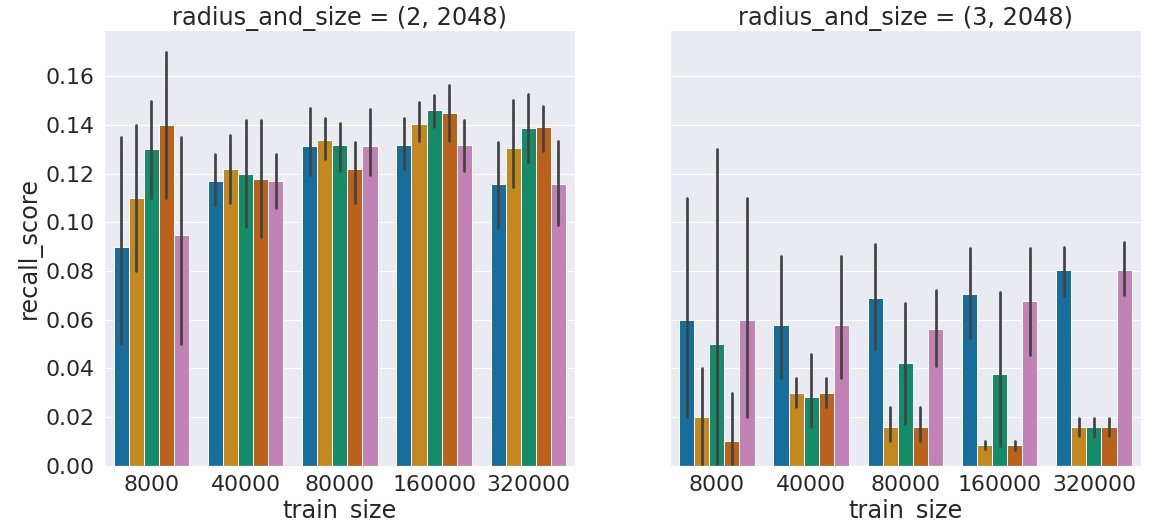
\includegraphics[scale = 0.4]{Images/DifferentMorgan1.jpg}
\end{subfigure}
\hfill\break
\begin{subfigure}{\textwidth}
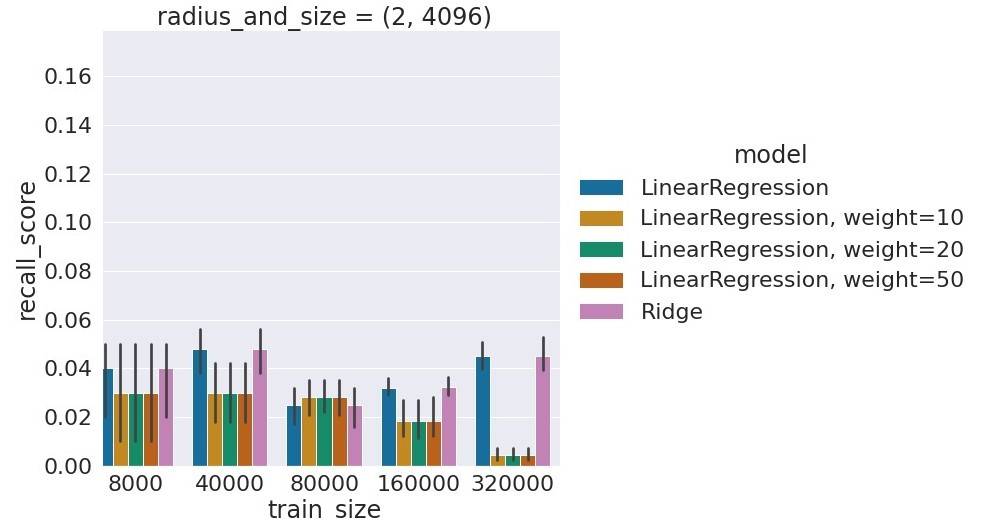
\includegraphics[scale = 0.55]{Images/DifferentMorgan2.jpg}
\end{subfigure}
\caption{Comparison of models trained on Morgan fingerprints}
\end{figure}


%Comparing radius 2 and 3 and size 2048 and 4096
\hfill\break
\subsection{Types of fingerprints}

As long as Morgan fingerprints are not the only one utilized in QSAR modelling, another type of fingerprints could be used for prediction. 
Thereby, atom pair fingerprints were generated for the dataset and used for training. 
Models, which were trained on Morgan and atom pair fingerprints, have showed comparable results (Fig. \ref{MvsAP}), and further work has been done using Morgan fingerprints.

\begin{figure}[H]
    \centering
    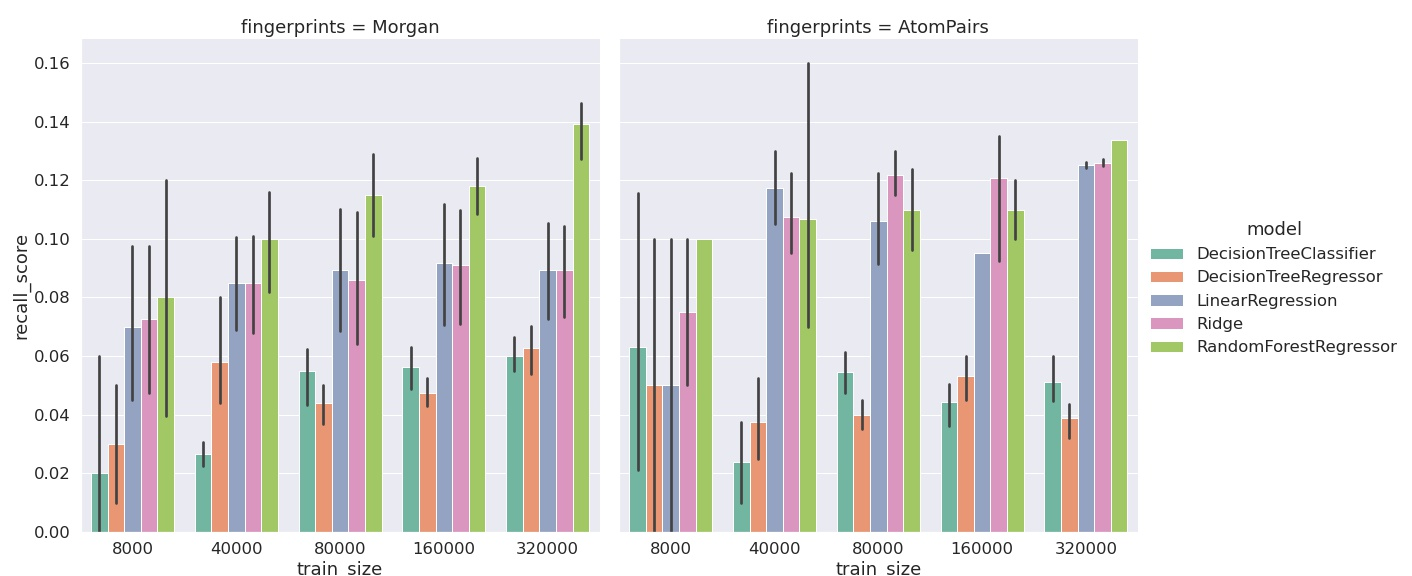
\includegraphics[width=\linewidth]{Images/MorganVSAtomPairs.jpg}
    \caption{Comparison of some models trained on Morgan and Atom pair fingerprints (4eiy)}
    \label{MvsAP}
\end{figure}



\hfill\break
\subsection{Comparing with docking}

Linear regression has been chosen as a single model for an iterative algorithm predicting docking scores of target 4eiy. 
It was one of the best performing models during the analysis, being one of the quickest one in training and prediction, and results given by the linear regression can be easily interpreted: according to the weight of each bit of the fingerprints it is possible to suggest which chemical substructures play significant role in attraction/repulsion between the binding site and a small molecule. 
Also, the quality of the linear regression can be improved at no cost by adding weights to molecules which are considered as docking hits.\\

Recall of the linear regression has already been compared with "dummy" regressors which give a random number from a unifrom or a gaussian distribution(Fig. \ref{Regressors}, Table \ref{recalls}).
The upper estimate should also be done through the use of the independent round of docking with effort=1 (Fig. \ref{linregVSdocking}).

\begin{figure}[H]
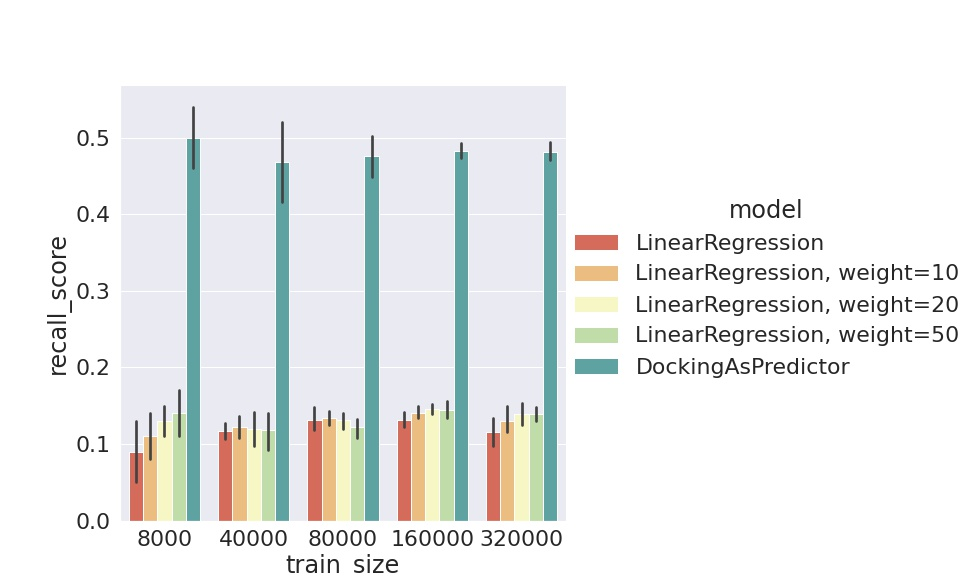
\includegraphics[scale = 0.45]{Images/LRvsD.jpg}
\caption{Models based on linear regression compared with docking}
\label{linregVSdocking}
\end{figure}

\section{Complex model}

\subsection{Determination of the best parameters}

\begin{figure}
    \centering
    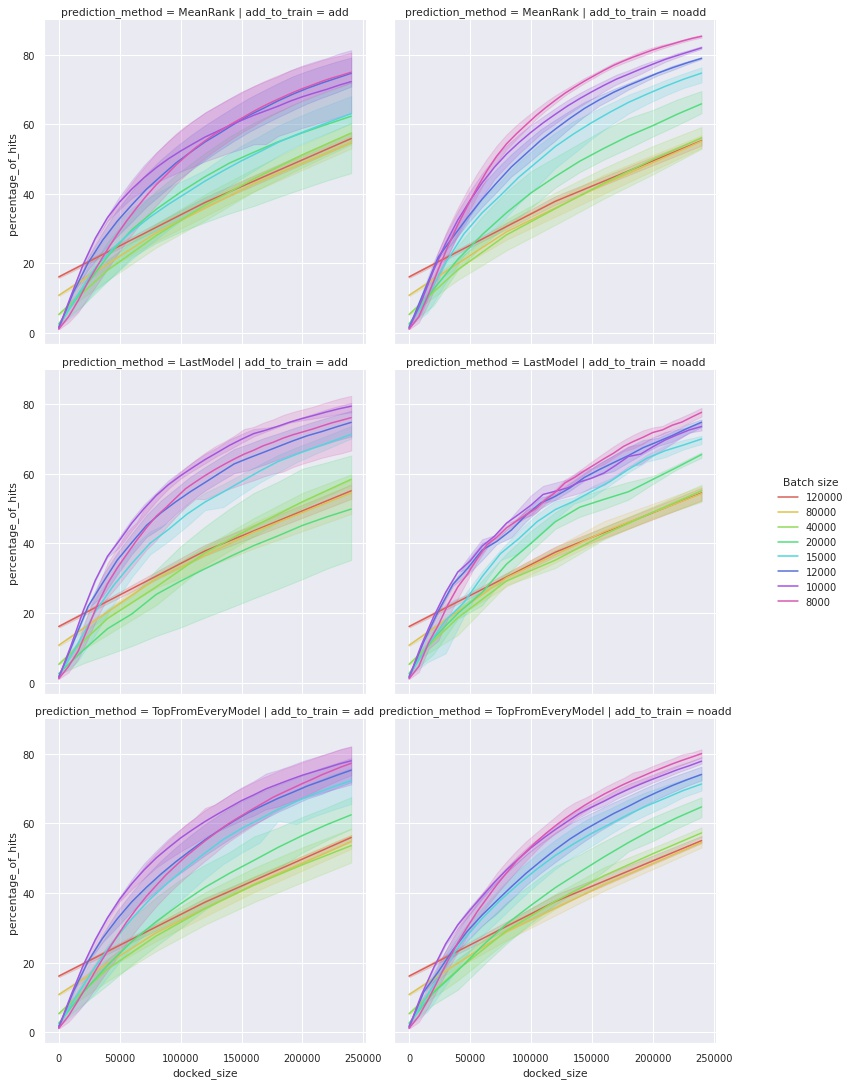
\includegraphics[width = \linewidth]{Images/LinregIterations.jpg}
    \caption{The portion of docking hits discovered by iterative algorithm depending on its parameters, the number of iterations and the amount of docked molecules}
    \label{4eiyLinReg}
\end{figure}

Iterative algorithm with "add" and "noadd" train set augmentation strategies, "LastModel", "MeanRank" and "TopFromEveryModel" complex model types was tested on the docking scores obtained for target 4eiy.
Firstly, linear regression was used as a single model. Depending on the batch size (the number of molecules docked during one iteration, the result of devision of 240,000 by the number of iterations), augmentation strategy and complex model, the algorithm has showed percentage of hits from 35\% to 85\%. The graphics are showed on the Fig.\ref{4eiyLinReg}.
Examination of all variations of the iterative algorithm has led to the conclusion that best performance gives the algorithm with "noadd" train set acquisition stratedy and "MeanRank" complex model.\\

Secondly, independent round of docking was utilized as a single model.
The percentage of hits discovered by the algorithm based on docking can give the upper bond for the effectiveness of the technique: no machine learning model can distinguish between hits and non-hits better than docking.
Hereby, iterative algorithm reaches values of about 80\% with 25\% of docked molecules when using docking as a single model, as seen at Fig \ref{docking}.\\

\begin{figure}[H]
    \centering
    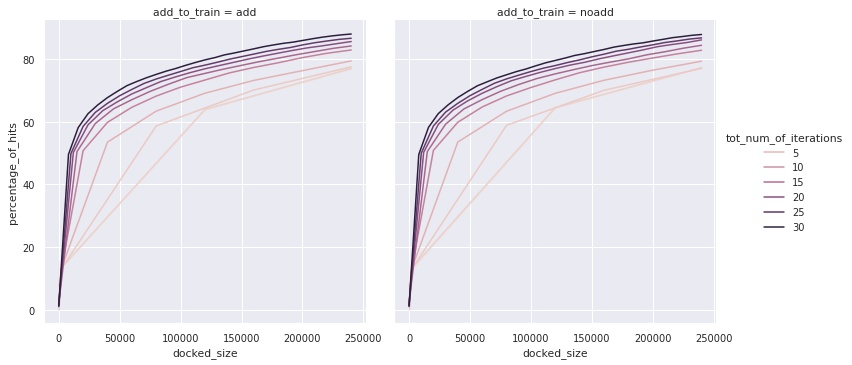
\includegraphics[width = \linewidth]{Images/DockingIterations.jpg}
    \caption{Performance of the iterative algorithm with docking as a single model}
    \label{docking}
\end{figure}

Thus, variation of the algorithm based on the linear regression can be considered as effective if the fraction of discovered hits will not differ much from 80\% with 25\% of docked molecules. 
Algorithm with best performing parameters meets these criteria.
That means that iterative algorithm based on the linear regression is an effective algorithm with correct choice of its parameters.\\

Besides, it it worth to notice difference common for all complex models depending on "add" or "noadd" strategy they use: when a certain number of iterations is reached, the quality of the algorithm with "noadd" strategy begins to deteriorate.
This can be explained by lower variety of single models in the iterative algorithm: when training set does consists partly of "old" molecules, model on next step does not differ from the one from the previous step.
The fewer molecules are added during the iterations, the less significant is the difference between models.
Thus, when number of iterations is big enough, models start to pick molecules in the same area of chemical space, ommiting higher part of the hits.
On the other hand, when all models are trained on the independent subsets of docked molecules, they show higher diversity.
That means that models prioritize separate fields of chemical space, which allow to gather more docking hits.\\

\subsection{Exploring the variety of the models in the algorithm}

The statement about higher variety of "noadd" models can be proved thanks to simplicity of a linear regression.
The 2048-dimensional space of coefficients of all trained models in the algorithm can be projected on plane using t-sne.
Result of projection is shown on \ref{tsne}. 
It allows to confirm the assumption about greater variety of models trained in iterative algorithm with "noadd" train set augmentation strategy.

\begin{figure}
\centering
\begin{subfigure}{\textwidth}
\centering
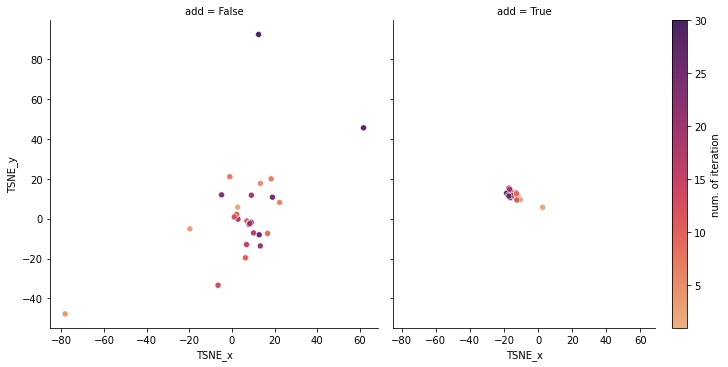
\includegraphics[scale = 0.50]{Images/LMtsne.jpg}
\caption{"LastModel"}
\end{subfigure}
\hfill\break
\begin{subfigure}{\textwidth}
\centering
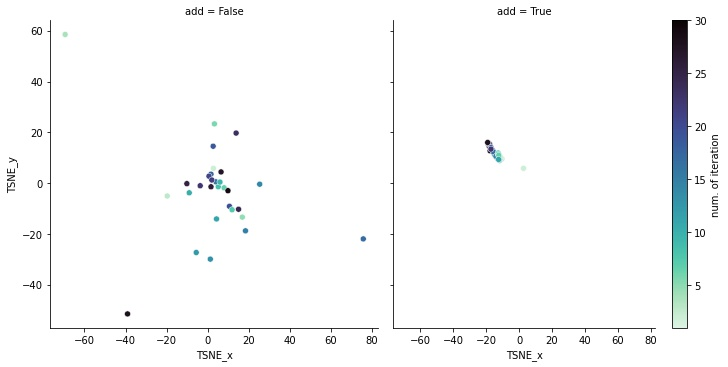
\includegraphics[scale = 0.50]{Images/TPEVtsne.jpg}
\caption{"TopFromEveryModel"}
\end{subfigure}
\hfill\break
\begin{subfigure}{\textwidth}
\centering
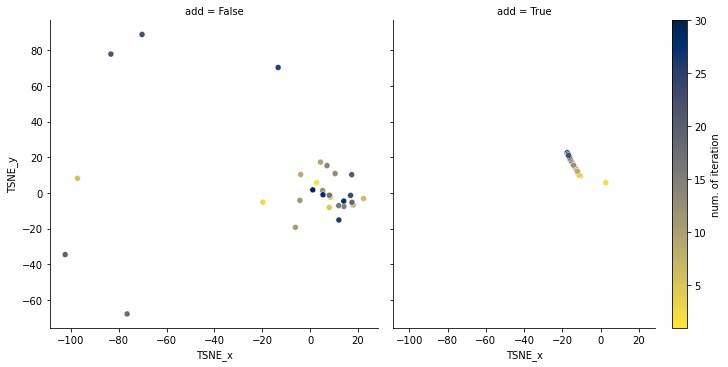
\includegraphics[scale = 0.50]{Images/MRtsne.jpg}
\caption{"MeanRank"}
\end{subfigure}
\caption{Comparison of varieties of model obtained when using "add" and "noadd" strategies}
\label{tsne}
\end{figure}

\subsection{Comparison of several models in the iterative algorithm}

Several machine learning models were used to build an iterative algorithm in order to determine how strongly recall affects the number of hits found by the algorithm. The best performing parameters of the algorithm were set: a 8,000-compounds batch, "MeanRank" complex model and "noadd" acquisition strategy.\\

Suddenly, the model with best recall score has performed worst of all, but still the fraction of obtained docking hits is still high.
The result shows that a model with best recall score evaluated may not be the best one for an iterative algorithm. \\

\begin{figure}[H]
\centering
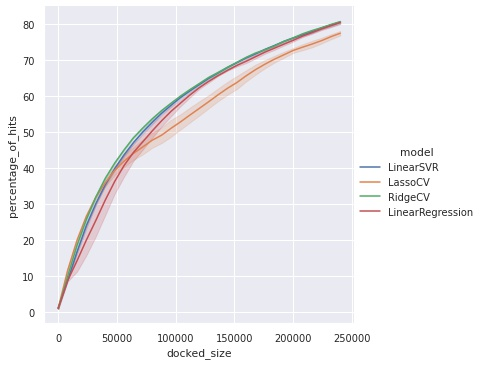
\includegraphics[width = 0.7\linewidth]{Images/5ztyModelsIterations.jpg}
\caption{The percentage of hits obtained by iterative algoruthm based on several machine learning models. Results are averaged by two independent runs of the algorithm.}
\label{}
\end{figure}

\subsection{Comparison of the iterative algorithm with exhaustive docking}

As already mentioned above, iterative algorithm shows best performance with "noadd" train set acquisition strategy and "MeanRank" complex model.
The comparison between the fractions of hits found by iterative algorithm, with best parameters, with docking,  linear regression or dummy random regressor as a simple model, and also their derivative is shown on Fig. \ref{best}. 


\begin{figure}[H]
\centering
\begin{subfigure}{0.85\textwidth}
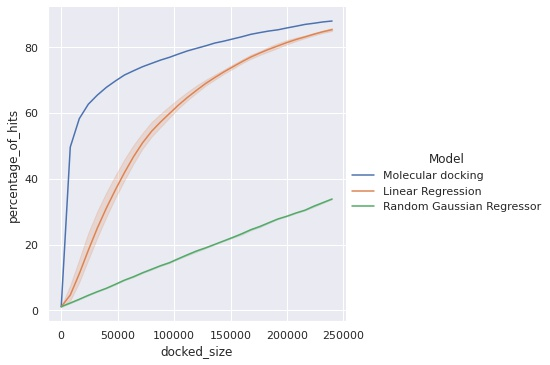
\includegraphics[width=0.9\linewidth]{Images/4eiyPercentageOfHits.jpg} 
\caption{Percentage of hits obtained depending on the number of docked molecules}
\label{best1}
\end{subfigure}
\begin{subfigure}{0.85\textwidth}
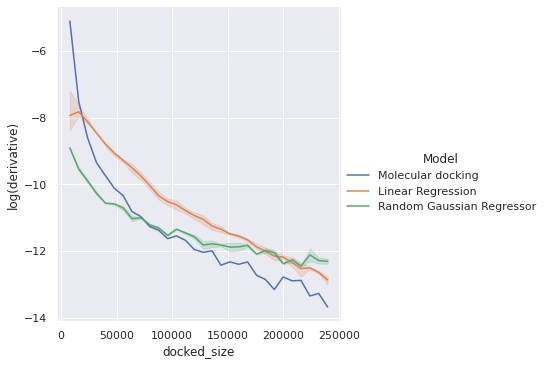
\includegraphics[width=0.9\linewidth]{Images/4eiyDerivative.jpg}
\caption{Derivative of \ref{best1} in logarithmic scale}
% \label{fig:subim2}
\end{subfigure}

\caption{Best performing variation of iterative algorithm compared with docking and dummy regressor. The parameters of the algorithm are: batch size = 8000 molecules, complex model = "MeanRank", augmentation strategy = "noadd"}
\label{best}
\end{figure}


The graph shows that if the size of docked molecules reaches 25\% of the set, then the number of hits predicted by linear regression and docking differs by less than 3\%, what can be considered as an insignificant loss of predictive ability.
It is also possible to compare the efficiency and spent time for docking and an iterative algorithm based on linear regression.
Since the prediction time by linear regression is negligible compared to the docking time, it can be neglected when estimating the time spent. 
Hence, 4-fold reduction of time allows to receive 85\% of docking hits and 10-fold reduction - 60\% of them.\\

According to the derivative plot, when the amount of docked molecules reaches 200,000, the recovery rate of linear regression-based algorithm becomes lower than one of random search.
That means that after a certain step of the algorithm, it does not bring benefits comparing to picking molecules randomly.
Unfortunately, there is no stop criteria to make from this knowledge because without docking the whole library it is impossible to distinguish between docking hits and non-hits.\\

Still, the stop criteria can be established using median score of docked molecules. 
As seen on the Fig.\ref{scores}, median score of linear regression-based algorithm drops firstly, and recovers as long as compounds with good scores are depleted. 
Comparison with median score after the first iteration can be used as a stop criteria: as soon as the latest batch of docked molecules has a median score higher than the first batch, the algorithm should be stopped.
\begin{figure}[H]
\centering
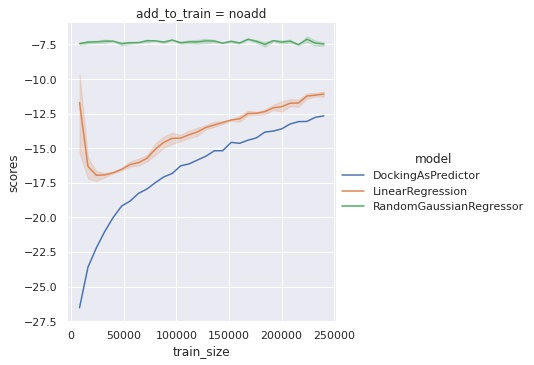
\includegraphics[width = 0.85\linewidth]{Images/4eiyScoresBest.jpg}
\caption{Median scores of predicted hits. The parameters of the algorithm are: batch size = 8000 molecules, complex model = "MeanRank", augmentation strategy = "noadd"}
\label{scores}
\end{figure}

